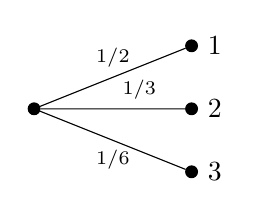
\begin{tikzpicture} [
  level distance=2cm,
  grow'=right,
  level 1/.style= {sibling distance=0.8cm},
  solid node/.style= {circle,draw,inner sep=1.5,fill=black},
]
\node (0) [solid node] {}
  child {node (A1) [solid node,label=right: {$1$}] {} edge from parent node [above] {\scriptsize $1/2$}}
  child {node (A2) [solid node,label=right: {$2$}] {} edge from parent node [above right] {\scriptsize $1/3$}}
  child {node (A3) [solid node,label=right: {$3$}] {} edge from parent node [below] {\scriptsize $1/6$}};
\end{tikzpicture}
\qquad
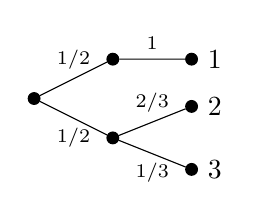
\begin{tikzpicture} [
  level distance=1cm,
  grow'=right,
  level 1/.style= {sibling distance=1cm},
  level 2/.style= {sibling distance=0.8cm},
  solid node/.style= {circle,draw,inner sep=1.5,fill=black},
]
\node (0) [solid node] {}
  child {node (A1) [solid node,label=right: {}] {} 
  child {node (B1) [solid node,label=right: {$1$}] {} edge from parent node [above] {\scriptsize $1$}}
  edge from parent node [above]{\scriptsize $1/2$}
    }
  child {node (A2) [solid node,label=right: {}] {} 
  child {node (B2) [solid node,label=right: {$2$}] {} edge from parent node [above] {\scriptsize $2/3$}}
  child {node (B3) [solid node,label=right: {$3$}] {} edge from parent node [below] {\scriptsize $1/3$}}
  edge from parent node [below] {\scriptsize $1/2$}
  };
  
\end{tikzpicture}
